\chapter{Background}
    \label{chap:background}

   This chapter will cover the necessary technical background regarding Inter Component Communication. It will first give an overview of important concepts of the Android Operating System. Following that, we will explain what components and permissions are in Android, and then go on to discuss in detail Inter Component Communication, which is a type of IPC specific to this OS. Subsequently, we explore the various types of vulnerabilities related to Inter Component Communication. 
    
    \section{Basics of the Android Operating System}
        \label{sec:android_basics}
    
    In Android, each application is by default assigned a unique user ID known only by the OS. The files of an app can only be accessed by a Linux user with the same ID as that of the app. Moreover, each app runs in its own process by default, and each process runs in its own virtual machine \cite{android_app_fundamentals}. Consequently, each Android application runs in its own sandbox, which enhances the security of the system, as apps are generally separated from each other.
    
    Throughout the continuous development of Android, the API is modified to introduce new features and improve security or performance. Therefore, in order to identify each incremental version of the API, a unique integer is assigned to each version or level. Over the years, there have been changes to the API that improved software security, and therefore some vulnerabilities are harder or impossible to exploit in current API levels.
    
    The manifest of an Android app is an XML file that gives the system information about the app’s structure, capabilities and needs. All Android app components, except broadcast receivers, need to be declared in the manifest file, and for each component you can define permission requirements and the capabilities of the component \cite{android_app_fundamentals}. Moreover, the developer can say in the manifest file what hardware or software system features the app uses, whether those features are required, and what is the minimum API level the app requires. For example, an app would not be installed on a device if the app’s manifest said it required a microphone and the mobile device did not posses microphone hardware.  Components will be explained in detail later in section \ref{sec:android_components}, and permissions in section \ref{sec:permissions}.
    
    The manifest also specifies the target SDK version of the app, which refers to the API version for which the is built to run on. Android apps can run on devices with a different API version as well.
    
    \section{Android Components}
        \label{sec:android_components}
        
    Android mobile apps are made up of logical building blocks called components. A component is an entity which allows the user or the operating system to access the application \cite{android_app_fundamentals}. Therefore, a component does not necessarily correlate with other computing concepts such as processes or threads. When any component of an app needs to be run, the system starts a process for that app. There are four types of components in Android: activities, services, broadcast receivers and content providers. We will detail these in the rest of section \ref{sec:android_components}
    
    \subsection{Activities}
        \label{subsec:activities}
        
    Activities represent the individual app UI screens through which a user interacts with the app. For example, a news aggregator application might have an activity for viewing a list of news articles.
    
    Activities are used by the operating system to keep track of what the user sees on screen, what information they are interested in, and the information of minimized apps that might be needed later \cite{android_app_fundamentals}.
    
    \subsection{Services}
        \label{subsec:services}
        
    Services are components used for running long-term operations in the background. Importantly, a service does not represent a separate process or thread, but an interface for the system to let the app work in the background \cite{whats_is_a_service}. A service does not have a user interface itself. Examples of the usage of services include VPN apps that maintain a VPN connection in the background.
    
    There are three types of services: foreground services, which perform tasks that are noticeable to the user and must display a notification, background services, which do things that are not noticeable to the user, and bound services, which act as servers responding to requests made by client components \cite{services_overview}.
    
    \subsection{Broadcast Receivers}
        \label{subsec:receivers}
        
    Broadcast receivers are components that an app uses to receive system wide broadcasts. These broadcasts are messages sent by the operating system or by other apps. Applications can react to various events by using broadcast receivers. For example, the system can send a broadcast to let apps know that the device’s battery is low or that airplane mode has been activated. An app can use a broadcast receiver to listen for an event even when the app is not running. Broadcast receivers do not have a user interface but can display notifications in the device’s status bar. In addition, it is worth noting that they do not have to be declared in the manifest but can be created programmatically as well.
    
    There are three types of broadcasts:
    \begin{itemize}
        \item Normal broadcasts – These are sent to all receivers at the same time, and each receiver can react independently of other receivers.
        \item Ordered broadcasts – These are sent to receivers one at a time. Unlike with a normal broadcast, the receiver currently processing the broadcast can change what information the broadcast contains, and can even cancel the broadcast, so that it will not be sent to further receivers \cite{broadcasts_overview}. Broadcast receivers can be registered with a certain priority for getting broadcasts.
        \item Sticky broadcasts – They are persistent broadcasts, they remain after they have been broadcast to all receivers and are re-broadcast to any new receivers. They have been deprecated since API level 21, because they are very insecure \cite{sticky_broadcast}.
    \end{itemize}
    
    \subsection{Content Providers}
        \label{subsec:content_providers}
        
    Content providers are interfaces through which apps can access data stored in persistent storage such as a remote server, an SQL database or local file storage. A provider can be used by components of the same app or by components of other apps. Therefore, they are used by the system to manage access to shared data. Content providers can restrict access to the data to apps with certain permissions and give temporary access to certain files only \cite{android_app_fundamentals}.
    
    \section{Permissions}
        \label{sec:permissions}
        
    Android follows the principle of least privilege. This means that, by default, each app only has access to the resources that it needs to complete its job. This principle is enforced through a system of permissions, meaning that an application can only access sensitive data, system features or components of other applications if it possesses the necessary requirements \cite{permissions_guide}. For instance, an application needs the correct permission if it wants to access the user’s contacts or the device’s camera.
    
    The developer can protect the components of an app with permission requirements by adding an android:permission tag in the manifest file. These elements can be added once for the whole application, or on a per component basis.
    
    \subsection{Types of permissions}
        \label{subsec:types_of_permissions}
        
    There are four types of permissions, based on the level of protection they allow:
    
    \begin{itemize}
        \item Normal permissions – Permissions for unimportant resources, such as the permission to set the time zone \cite{permissions_guide}. They are granted automatically at install time.
        \item Dangerous permissions – These permissions are for important resources such as private user information, or that can affect the state of the system or of other apps. The user needs to give explicit permission in the app to utilise these resources.
        \item Signature permissions – These are special permissions designed for use among a group of apps created by the same developer. An app is automatically granted a signature permission at install time only if it is signed by the same certificate as the app that defined the permission. The certificate does not have to be signed by a certificate authority, they can be self-signed by the developer. Their purpose is to identify the author of an app \cite{define_custom_permission}.
        \item Signature or System permissions - a deprecated type of permission since API level 23 \cite{manifest_permissions_element}. It is automatically granted only if the app is signed by the same certificate as the app that declared the permission or if the app is in the system folder. Apps in the system folder are installed by the mobile device’s vendor.
    \end{itemize}
    
    \subsection{Custom permissions}
        \label{subsec:custom_permissions}
        
    Applications can declare their own permissions. These can be used to restrict access to components of an application, or protect broadcasts of that app. This is done by declaring a permission in the manifest file of the app.
    
    \lstinputlisting[language={xml}, label={lst:custom_permission}, caption={A declaration of a custom permission in an Android manifest.}]{./listings/custom_permission.xml}
    
    \section{Inter Component Communication}
        \label{sec:inter_component_communication}
    
    So far, we have seen that each Android application runs in its own sandbox, and by default can not see what other applications are doing. Sometimes, we need the system to communicate with the apps, and applications can enrich the users experience by collaborating. Moreover, an application component can be used by other apps to provide extra functionality. For example, a browser lets you select which social media or messaging app to use for sharing a link.
    
    Intents are a class in the Android API that are used as messages for communication between application components. More specifically, intents are used to start new activities, start and stop services, bind or unbind a component to a service, and they also represent the broadcasts that are sent to receivers.
    
    \subsection{Exported Components}
        \label{subsec:exported_components}
        
    By default, app components are not accessible to outside apps through intents. However, a component can be exported and thus receive intents from other applications. To export a component, you can set the \lstinline|<exported>| tag in a component in the app’s manifest to true. However, if the component has an intent filter defined in the manifest, the component will become automatically exported unless the exported tag is explicitly set to false. Intent Filters will be fully explained in section 3.5.3.
    
    Further complicating component exportation is that developers can configure an application to use the same Android User ID as other applications created by them. This means these apps can run in the same process, and they can access each other’s components regardless of the exported tag or the presence of intent filters, as can be seen in figure \ref{fig:component_exportation}
    
    \begin{figure}[h]
        \centering
        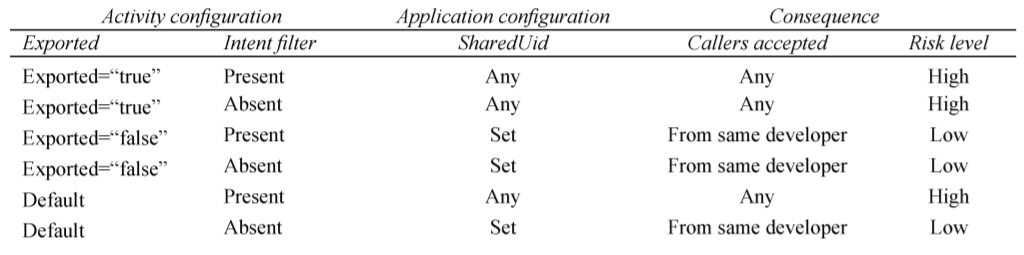
\includegraphics[width=1\textwidth]{graphics/component exportation.PNG}
        \caption{Exportation of components in various circumstances. Taken from \cite{2013_permission_leaks_study}.}
        \label{fig:component_exportation}
    \end{figure}
    
    \subsection{Explicit Intents}
        \label{sec:explicit_intents}
        
    Explicit intents directly specify the application that should receive the intent and handle it. This is done by setting either the package name of the receiving application, or the full name of a component of said app \cite{intents_and_intent_filters}. Explicit intents can contain other information, such as data or the intended action to be performed, as you can see in Listing \ref{lst:explicit_intent}.
    
    Using an explicit intent means that only the targeted app or component can receive the intent. Explicit intents are usually used for communication between components of the same app, such as when one activity starts another when the user clicks a button. That being said, explicit intents can be used to start components of other apps as well. As explained in subsection \ref{subsec:exported_components}, an app component must be exported so that other apps can send explicit intents to it.
    
    \lstinputlisting[language={java}, label={lst:explicit_intent}, caption={Kotlin code to make an explicit intent, add data to it and start an activity with it}]{./listings/explicit_intent.kt}
    
    \subsection{Implicit Intents}
        \label{sec:implicit_intents}
        
    Unlike explicit intents, implicit intents do not directly specify what application or component it should be sent to. Instead, the Android system decides who to send it to based on the information in the intent and what other components have declared they can handle.
    
    A component defines what intents it can handle by specifying Intent Filters in the manifest file, with an example in Listing \ref{lst:intent_filter}. An Intent Filter defines the type of intents an application can handle. A filter can say what actions the component can perform, what intent categories it accepts, the MIME data types it accepts or the kind of URI resources it can handle. A component may declare multiple Intent Filters, and it is recommended that this is done for each task the component can do \cite{intents_and_intent_filters}.
    
    \lstinputlisting[language={xml}, label={lst:intent_filter}, caption={Declaration of an intent filter that the intent in Listing \ref{lst:implicit_intent} will match.}]{./listings/intent_filter.xml}
    
    When an implicit intent is sent, like you can see in Listing \ref{lst:implicit_intent}, the Android System compares its attributes against all intent filters of all components. For the intent to be matched with a filter, three tests are performed: the Action test, the Category test, and the Data test \cite{intents_and_intent_filters}. In order to pass the Action test, the Intent’s action must be amongst the actions of the filter. It passes the Category Test if all of its categories are found in the filter’s declaration, and the Data Test is passed if the data URI or MIME type of the intent matches one of the data elements in the filter. If the component has multiple filters, the intent only needs to match one of them for it to be passed to the component.
    
    \lstinputlisting[language={java}, label={lst:implicit_intent}, caption={Kotlin code to make an implicit intent, add data to it and start an activity with it}]{./listings/implicit_intent.kt}
    
    If only one intent filter matches the implicit intent, the operating system will start that filter’s component automatically. However, if there are multiple matches, a dialog will be displayed to the user so they can manually select the component to handle the intent.
    
    For example, if there are multiple browsers installed on a device, and within an app the user clicks on a web link, they will then see an Android dialog letting them choose what browser to use to open that page. This is because the parent app sent an implicit intent, and all browsers had filters that matched with the intent.
    
    \section{Inter Component Communication Vulnerabilities and Attacks}
        \label{sec:icc_vulnerabilities_and_attacks}
        
    In this section, we will explain how the way components communicate using Intents can be exploited by attackers, and what developers can do to fix these vulnerabilities.
    
    Most of the vulnerabilities that will be explored in this project happen due to the misuse of implicit intents or intent filters. Because implicit intents do not directly state what component they target, it is possible that an intent is delivered to a malicious app. Moreover, an attacker could create malicious intents that could launch other components in ways that could compromise the victim app.
    
    \subsection{Unauthorised Intent Receipt}
        \label{subsec:unauthorised_intent_receipt}
        
    The Android documentation recommends that explicit intents are used for intra-app communication, and implicit intents for inter-application communication \cite{intents_and_intent_filters}. However, developers sometimes use implicit intents to start a component within the same app. An attacker can make an app with an intent filter designed to match with said implicit intents, which can direct the intent to the malicious application. When receiving an intent, a component can read all of its data. Therefore, even if the implicit intent is meant for external use, if the developer puts sensitive information in it, that data could be intercepted.
    
    In general, vulnerabilities against this class of attacks are fixed by using explicit intents instead of implicit intents in order to send broadcasts, start activities or services or grant access to a content provider \cite{2010_icc_paper}. Another way to mitigate these attacks is to not put sensitive information in implicit intents.
    
    The rest of subsection \ref{subsec:unauthorised_intent_receipt} explains various types of the Unauthorised Intent Receipt attack.
    
    \subsubsection{Broadcast Theft}
        \label{subsubsec:broadcast_theft}
    
    When a broadcast is sent, the sender does not receive any indication of what components have received that broadcast. A malicious app could register a broadcast receiver with as many intent filters as possible to listen to many public broadcasts \cite{2010_icc_paper}. The malware would be able to read the data in the broadcasts without the user knowing it, and could therefore be used as spyware. Moreover, if an implicit intent is used for a broadcast meant for an app’s internal use, that broadcast will be sent to any receiver on the device with a matching filter.
    
    Ordered broadcast are sent to receivers one at a time, as explained in subsection \ref{subsec:receivers}. The use of ordered implicit broadcasts can not only enabled eavesdropping as described above, but denial of service and man in the middle attacks as well \cite{2010_icc_paper}. A malicious app could register a broadcast receiver with a very high priority to ensure it is the first to receive it. It could extract the data from the broadcast, and then abort the broadcast, ensuring the intended receivers do not get it and thus perform a Denial of Service attack. Otherwise, the malicious receiver could replace the original data with malicious data, and perform a Man In the Middle attack. This could be used to corrupt data or crash other applications.
    
    When making a broadcast, the developer can specify the permission that a broadcast receiver needs to have in order to be able to get it. This can be used to guard against Broadcast Theft. A developer can declare their own custom permission, as seen in section \ref{sec:permissions}, which must be obtained by receivers to be able to get broadcasts sent by the developer's app. 
    
    However, if the developer does not set the protection level of the permission, it will default to "normal", and the malware will get it automatically at install time. The developer can set the protection level to "dangerous", meaning the malware needs to ask the user to grant that permission. This is quite secure, but a careless user may still grant it. The most secure protection level for the custom permission is "signature", but if the private key of the certificate is not stored securely, it can be stolen and be used to sign the malware, which would be able to get the permission. In order to make broadcast theft impossible, the broadcast should be sent as an explicit intent, or as an implicit intent which specifies the package of components that can receive it \cite{2010_icc_paper}. Other ways for a developer to guard against these attacks is to not put sensitive information in a broadcast unless necessary.
    
    \subsubsection{Activity Intent Hijacking}
        \label{subsubsec:activity_hijacking}
        
    In this type of attack, a hacker takes advantage of the use implicit intents so that a malicious activity is launched instead of the intended one, by registering the right intent filters for their malicious activity.
    
    In a sophisticated version of this attack, the attacker could use phishing to steal user credentials \cite{2010_icc_paper}. For example, consider an application with a log in screen. If that application uses an implicit intent to start the Log In activity, a hacker could create an identical looking Log In activity in their app. They could then use an identical intent filter for their fake activity. This means that the implicit intent will match both the fake Log In activity and the legitimate one as well, and thus prompt the user to choose between them. The attacker can give a confusing or identical name to their malware, or make the icons of the two apps similar in order to make the user choose the malware. The unaware user would then type in their credentials on the fake Log In screen, which could then be sent to the hacker.
    
    This type of attack is most dangerous when it intercepts implicit intents meant to launch an activity within the same app. This is because it disrupts the workflow of that app, and the attacker can get data that should be private.
    
    \subsubsection{Service Intent Hijacking}
        \label{subsubsec:service_hijacking}
        
    This type of attack is similar to the Activity Intent Hijacking attack, but it concerns the malicious start of unwanted services. If a mobile application uses an implicit intent to start a service, then the Android system will search for services with intent filters that match the intent. A key difference between activities and services is that when multiple services have filters matching the same intent, then the OS chooses a service to start at random \cite{startService}, the user does not get to choose. This, combined with the fact that services give at most a notification in the Android status bar, means that it is harder for the user to be aware of this attack.
    
    Once the malicious service is started, a multitude of things can happen. It could steal any sensitive data in the intent and lie about completing the intended task. Even more dangerous is the scenario where the implicit intent is used start a bound services, which can return information to the client components more easily and frequently. Thankfully, since Android 5.0 it is impossible to start a bound service with an implicit intent \cite{bound_services}, and therefore we have not covered Intent Hijacking for bound services. A malicious service could return false information to clients, and this could be used to crash other apps and thus perform a Denial of Service Attack, pollute other components with fake data or manipulate the client components to perform other attacks \cite{2010_icc_paper}.
    
    To give an example, consider a messaging app like WhatsApp. This app would use a service for making periodical backups of the user’s messages. If it used an implicit intent to start this service, an attacker could make a service in their app with a matching intent filter. The malicious service could be started at random instead of the legitimate one. This service could then get access to the user’s messages and upload them in the background to the attacker’s server. The malicious service could be hidden in an app that appears to have an unrelated functionality, and thus be hidden.
    
    \subsubsection{Content Provider URI Hijacking}
        \label{subsubsec:provider_uri_hijacking}
        
    We have discussed that intents can transmit data using a URI. These URIs can point to data stored using a Content Provider. We have also explained that permissions can be set on a per component basis. However, when declaring a Content Provider in the manifest file, the developer can set the \lstinline|android:grantUriPermissions| tag of the \lstinline|<provider>| element to true. This means that the content provider can allow temporary access to data linked to in a URI for a component that does not otherwise have the permission required by the provider. Therefore, external apps can access the content provider, even if the provider is not exported and is thus not accessible by external apps in general.
    
    In order to do this, the intent that transmits the URI link must have the \lstinline|FLAG_GRANT_READ_URI_PERMISSION| or \lstinline|FLAG_GRANT_WRITE_URI_PERMISSION| flags added to it. If this intent is an implicit intent and is intercepted by a malicious component, then that component can read the data and perhaps modify it. This attack can put private information, such as debit card information or a phone number, in the hands of attackers.
    
    \section{Intent Spoofing}
        \label{sec:intent_spoofing}
        
    While the Intent Hijacking attacks that we have detailed worked by accidentally activating a malicious component when an intent is intercepted, Intent Spoofing attacks happen when a victim component is unexpectedly activated by an attacking component using an Intent. Often, this attack targets components that are not meant to be accessible outside of their apps, but because they have an intent filter and the \lstinline|<exported>| tag is not set, they are exported automatically. Because exported components are accessible to other apps, the attacker can create an explicit intent targeting it and does not need to worry about having to match intent filters. The developers are usually unaware of this.
    
    This attack is dangerous because components often extract information from the intents they receive. An Intent Spoofing attack could insert malicious information into the victim component. The attacker could send invalid information to crash the victim’s app (a DoS attack), corrupt the user’s data, or inject commands to retrieve data. Often, the launch of an activity, service or broadcast receiver leads a change in the application’s state \cite{2010_icc_paper}, even if the victim component takes no input from the intent. And since activities and services can return information to the component that activated them, they could leak sensitive information. This attack is often done against components that were not meant to be accessible to other apps, and these components are thus less likely to check the input data of the intent or make sure they do not return private data.
    
    Developers can secure their application from this class of attacks in a number of ways  \cite{2010_icc_paper}. First, they should not declare intent filters for internal components, and they should use explicit intents to launch them. Secondly, if they need to use intent filters for internal components, they should explicitly declare them as not exported in the manifest. Thirdly, they can protect components with permissions of various types. Fourthly, state-changing operations should not be done in exported components. And finally, developers should make sure that exported components do not return information that should be private.
    